\subsubsection{Zielsetzung und Anforderungen}

Ziel des Projekts ist die Entwicklung einer Platine, die EEG-Signale generieren und über vier Kanäle analog ausgeben kann. Dabei soll ein benutzerfreundliches System entstehen, das sich insbesondere für den Einsatz im Unterricht eignet und dort die Funktionsweise von EEG-Signalen veranschaulichen kann.

Die Signalparameter sollen über eine Weboberfläche konfigurierbar sein, ohne dass eine zusätzliche Softwareinstallation auf dem Computer erforderlich ist. Die Oberfläche wird über die integrierte WLAN-Schnittstelle des Mikrocontrollers bereitgestellt.

Hardwareseitig übernimmt ein Mikrocontroller die Generierung der Signale, die anschließend über einen Digital-Analog-Wandler (DAC) ausgegeben werden. Der DAC soll eine hohe Auflösung und Genauigkeit bieten, um eine realistische Darstellung der EEG-Signale zu ermöglichen.

Zur Nachbearbeitung der DAC-Ausgabe wird ein Operationsverstärker als aktiver Tiefpassfilter mit einer Verstärkung von 1 verwendet. Dieser dient der Glättung des Signals und der Reduktion von Rauschen. Da EEG-Signale typischerweise im Mikrovolt-Bereich liegen, wird das Ausgangssignal im Millivolt-Bereich erzeugt und anschließend mittels eines Spannungsteilers im Verhältnis 1:1000 auf den µV-Bereich herunterskaliert.

Die Stromversorgung der Platine erfolgt über eine USB-Schnittstelle. Die Generierung und Ausgabe der Signale soll dabei in Echtzeit erfolgen.



\subsubsection{Komponentenübersichet}

Die wichtigsten Komponenten der Platine sind:

\begin{itemize} 
    \item \textbf{Mikrocontroller:} ESP32-S3 16R8 – zur Signalverarbeitung und Bereitstellung der Weboberfläche. 
    \item \textbf{Digital-Analog-Wandler (DAC):} DAC8412FPZ – zur präzisen Ausgabe der generierten EEG-Signale auf vier Kanälen. 
    \item \textbf{Operationsverstärker:} TL071CDR – dient als aktiver Tiefpassfilter zur Glättung der Ausgangssignale. 
    \item \textbf{Spannungsversorgung:}
    \begin{itemize}
        \item NCV1117DT50RKG – LDO-Spannungsregler für 5 V
        \item TL7660CDGKR – Ladungspumpe zur Erzeugung einer negativen Spannung
        \item TLV75733PDRVR – LDO für 3.3 V Betriebsspannung
        \item TS4061AILT-1.25 – eine stabile 1{,}25\,V-Referenzspannung        \item 
    \end{itemize}
\end{itemize}

Als Mikrocontroller kommt der ESP32-S3 16R8 zum Einsatz. Dieser bietet mit seinen zwei Kernen die Möglichkeit, die Weboberfläche auf einem Kern und die Signalverarbeitung auf dem anderen Kern zu betreiben. Der integrierte Flash-Speicher von 16MB bietet ausreichend Platz für Firmware und Webinterface.

Zur analogen Ausgabe der Signale wird der DAC8412FPZ von Analog Devices verwendet. Dieser 12-Bit-DAC zeichnet sich durch hohe Genauigkeit und schnelle Signalverarbeitung aus. Er verfügt über vier voneinander unabhängige Ausgänge und wird über eine parallele Schnittstelle angesteuert, wodurch eine hohe Datenrate und eine quasi-echtzeitfähige Signalübertragung gewährleistet sind.

Die analoge Nachbearbeitung der Signale erfolgt durch einen Operationsverstärker mit integriertem aktiven Tiefpassfilter. Dieser glättet die DAC-Ausgabe und reduziert hochfrequentes Rauschen.

Zur Erzeugung der notwendigen Versorgungsspannungen kommen ein LDO für 5V, ein negativer LDO, sowie eine Ladungspumpe zur Generierung der negativen Spannung zum Einsatz. Diese sind notwendig, um eine symmetrische Versorgung für den Operationsverstärker bereitzustellen.

\subsubsection{Schaltungsdesign}
\subsubsection{Gesamtüberblick}
\begin{figure}[H]
    \centering
    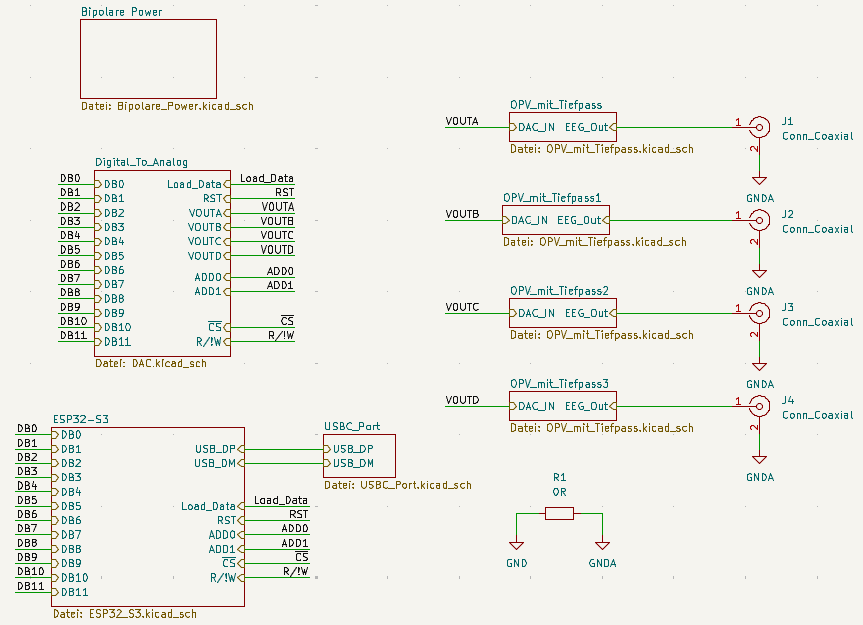
\includegraphics[width=0.8\textwidth]{bilder/Platine_gesamt.png}
    \caption{Gesamtübersicht der Platine}
    \label{fig:gesamtuebersicht}
\end{figure}
Die Platine ist in mehrere Funktionsblöcke unterteilt, die jeweils für spezifische Aufgaben zuständig sind. Diese Blöcke sind:
\begin{itemize}
    \item \textbf{Mikrocontroller-Block:} Enthält den ESP32-S3 16R8, der die Signalverarbeitung und die Weboberfläche steuert.
    \item \textbf{DAC-Block:} Beinhaltet den DAC8412FPZ, der die digitalen Signale in analoge Signale umwandelt.
    \item \textbf{Operationsverstärker-Block:} Besteht aus dem TL071CDR, der als aktiver Tiefpassfilter fungiert.
    \item \textbf{Spannungsversorgungsblock:} Umfasst die LDOs und die Ladungspumpe zur Bereitstellung der benötigten Spannungen.
    \item \textbf{USB-Block:} Dient der Stromversorgung der Platine über eine USB-Schnittstelle.
\end{itemize}


